\documentclass[xcolor={table}]{beamer}
%\usetheme{Lapesd}
\usepackage{./sty/beamerthemeLapesd}

\usepackage{morewrites}

\usepackage[brazilian]{babel}	% coloca as coisas em portugues no sumário.
\usepackage[utf8]{inputenc}
\usepackage[T1]{fontenc}
\usepackage[scaled]{helvet}
\usepackage{amsthm}
\usepackage{ragged2e}
% \usepackage{subfig}
\usepackage[table]{xcolor}
\usepackage{ctable}
\usepackage{multicol}
\usepackage{multirow}
\usepackage{fancyvrb}
\usepackage{subcaption}
\usepackage{algorithm2e}
\usepackage{listings}
\usepackage{color}
\usepackage[font={scriptsize,it}]{caption}
\renewcommand{\lstlistingname}{Code}
\definecolor{lightgray}{rgb}{0.97,0.97,0.97}
\definecolor{lightred}{rgb}{1,0.7,0.7}

\lstdefinelanguage{cc}{
    language     = C++,
    morekeywords = {Array2D, __parallel__, Mask2D, Stencil2D}
}

\lstdefinestyle{highlight}{
    numbers=none,
    stepnumber=1,
    numbersep=-8pt,
    numberstyle=\small\color{black},
    basicstyle=\scriptsize\ttfamily\color{black},
    keywordstyle=\color{blue},
    commentstyle=\color{black},
    stringstyle=\color{black},
    numberstyle=\footnotesize\ttfamily\color{black},
    escapeinside={(*}{*)},
    tabsize=2,
    language=cc, %morecomment=[l][{\color[rgb]{0.1, 0.2, 0.8}}]{},
    %aboveskip=0.1in, % space before the caption
    %belowskip=0.1in, % space after listing
    captionpos=b,
    showstringspaces=false,
    %belowcaptionskip=1\baselineskip,
    %breaklines=true,
    %moredelim=[l][\color{blue}]{\#pragma},
    % backgroundcolor=\color{white}
}

\lstdefinestyle{base}{
    numbers=none,
    stepnumber=1,
    numbersep=-8pt,
    morekeywords={Array2D, \_\_parallel\_\_, Mask2D, Stencil2D}
    numberstyle=\small\color{black!40},
    basicstyle=\scriptsize\ttfamily\color{black!40},
    keywordstyle=\color{blue!40},
    commentstyle=\color{black!40},
    stringstyle=\color{black!40},
    numberstyle=\footnotesize\ttfamily\color{black!40},
    escapeinside={(*}{*)},
%     frame=none, %single
    tabsize=2,
    language=cc, %morecomment=[l][{\color[rgb]{0.1, 0.2, 0.8}}]{},
    %aboveskip=0.1in, % space before the caption
    %belowskip=0.1in, % space after listing
    captionpos=b,
    showstringspaces=false,
    %belowcaptionskip=1\baselineskip,
    %breaklines=true,
    %moredelim=[l][\color{blue}]{\#pragma},
    % backgroundcolor=\color{white!40}
    moredelim=**[is][\only<+>{\color{black}\lstset{style=highlight}}]{@}{@},
}

% \lstdefinestyle{highlight}{
    % keywordstyle=\color{red},
    % commentstyle=\color{green},
% }
% \lstdefinestyle{base}{
    % language={C++},
    % basicstyle=\color{black!40},
    % keywordstyle=\color{red!40},
    % commentstyle=\color{green!40},
    % moredelim=**[is][\only<+>{\color{black}\lstset{style=highlight}}]{@}{@},
% }

\newcommand{\Fw}{\textit{Framework}\xspace}
\newcommand{\fw}{\textit{framework}\xspace}
\newcommand{\Fws}{\textit{Frameworks}\xspace}
\newcommand{\fws}{\textit{frameworks}\xspace}

\newcommand{\pskel}{PSkel\xspace}
\newcommand{\mppa}{MPPA-256\xspace}

\graphicspath{{./figs/}}
\DeclareGraphicsExtensions{.pdf,.jpg,.png,.gif}

\def\signed #1{{\leavevmode\unskip\nobreak\hfil\penalty50\hskip2em
        \hbox{}\nobreak\hfil(#1)
        \parfillskip=0pt \finalhyphendemerits=0 \endgraf}}

\renewcommand{\footnotesize}{\tiny}

\newcommand{\mymacro}[1]{#1}

\addtobeamertemplate{block begin}{}{\justifying}

\captionsetup{labelformat=simple}
\captionsetup[table]{belowskip=0pt}

\title[PSkel-MPPA: Uma Adaptação do Framework PSkel]{
    % \textbf{Execução Energicamente Eficiente de Aplicações Estêncil com o Processador \textit{Manycore} MPPA-256}}
    \textbf{PSkel-MPPA: Uma Adaptação do Framework PSkel para o Processador
        Manycore MPPA-256}}
\author[Podesta Junior, E.]{Emmanuel Podestá Junior
    \linebreak\linebreak
    \scriptsize{Orientação: Márcio B. Castro (UFSC)}}
\date{21 Junho 2017}
\institute{Departamento de Informática e Estatística (INE)\\
    Universidade Federal de Santa Catarina (UFSC)\\
    \url{emmanuel.podesta@grad.ufsc.br}}

\begin{document}
\begingroup
    \makeatletter
    \setlength{\hoffset}{-0.5\beamer@sidebarwidth}
    \makeatother
    \begin{frame}[plain,t,noframenumbering]
        \titlepage
    \end{frame}
\endgroup

%=============================================================================================

\section{Introdução}

\begin{frame}\frametitle{Contexto}
    \subsection{Contexto}
    \begin{itemize}
        \item{Aplicações complexas podem sobrecarregar a CPU}
        \item{Arquiteturas auxiliares}
            \begin{itemize}
                \item{Ex.: Aceleradores}
            \end{itemize}
    \end{itemize}

    \begin{itemize}
        \item{\textbf{Computação de Alto Desempenho}}
            \begin{itemize}
                \item {CPU e aceleradores (GPUs, manycores)}
                \item {Maiores ganhos em desempenho}
            \end{itemize}
    \end{itemize}
    \begin{figure}
        \centering
        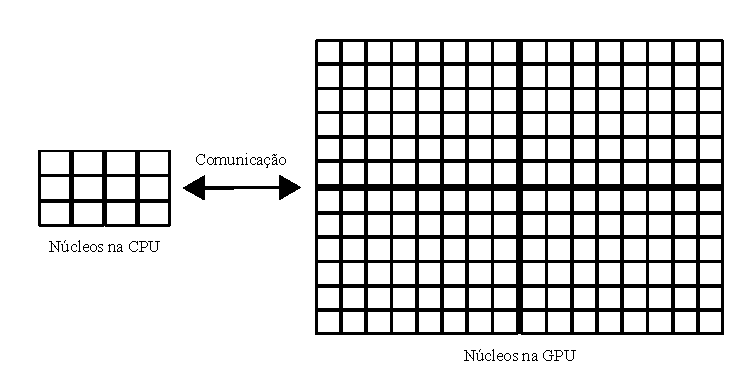
\includegraphics[width=0.90\textwidth]{figs/CPUGPU.pdf}
    \end{figure}
    \vfill
\end{frame}

\begin{frame}\frametitle{Contexto}
    \textbf{Dificuldades}
    \begin{itemize}
        \item {Programação Híbrida}
        \item {Comunicação entre CPUs e aceleradores}
        \item {Particionamento inteligente de tarefas}
    \end{itemize}
    \vfill
    % \textbf{Como podemos simplificar o desenvolvimento?}
\end{frame}

\begin{frame}\frametitle{Esqueletos Paralelos}
    \subsection{Esqueletos Paralelos}
    \textbf{Existem vários padrões paralelos ~\cite{mccool10}}
    \begin{itemize}
        \item {Map, reduce, scan, \textcolor{red}{estêncil}, entre outros.}
    \end{itemize}
    \begin{itemize}
        \item{Esqueletos abstraem os padrões paralelos}
        \item{Complexidade reduzida}
    \end{itemize}
    \textbf{\Fws baseados no padrão estêncil:}
    \begin{itemize}
        \item SkelCL ~\cite{steuwer11}
        \item SkePU ~\cite{enmyren10}
        \item PSkel ~\cite{pereira15}
    \end{itemize}
\end{frame}


\begin{frame}\frametitle{Padrão Estêncil}
    \subsection{Padrão Estêncil}
    \begin{itemize}
        \item {Cada célula da matriz é computada em função dos valores de seus vizinhos}
        \item {Computação Iterativa}
    \end{itemize}
    \begin{figure}
        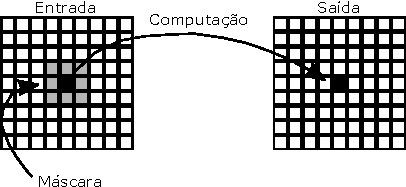
\includegraphics[width=0.6\textwidth]{26}
    \end{figure}
\end{frame}


\begin{frame}[fragile]
    \frametitle{Padrão Estêncil}
    \begin{lstlisting}[style=highlight, gobble=4]
	    void jacobi(int tsteps, int N, float *A, float *B){
		    int t, i, j;
		    float c1 = 0.2;

		    for (t = 0; t < tsteps; t++){
		    	for (i = 1; i < N-1; i++)
		    		for (j = 1; j < N-1; j++)
		    			B[i,j] = c1 * (A[i,j] + A[i,j-1] + A[i,j+1]
                          + A[i+1,j] + A[i-1,j]);

		    	for (i = 1; i < N-1; i++)
		    		for (j = 1; j < N-1; j++)
		    			A[i,j] = B[i,j]
		    }
	    }
    \end{lstlisting}
\end{frame}

\begin{frame}[fragile]
    \frametitle{Padrão Estêncil}
    \begin{lstlisting}[style=base, gobble=4]
	    @void jacobi(int tsteps, int N, float *A, float *B)@{
		    int t, i, j;
		    @float c1 = 0.2;@

		    @for (t = 0; t < tsteps; t++)@{
		    	@for (i = 1; i < N-1; i++)
		    		for (j = 1; j < N-1; j++)
		    			B[i,j] = c1 * (A[i,j] + A[i,j-1] + A[i,j+1]
                          + A[i+1,j] + A[i-1,j]);@

		    	@for (i = 1; i < N-1; i++)
		    		for (j = 1; j < N-1; j++)
		    			A[i,j] = B[i,j]@
		    }
	    }
    \end{lstlisting}
\end{frame}


\begin{frame}[fragile]
    \frametitle{Padrão Estêncil}
    \begin{lstlisting}[style=base, gobble=4]
	    void jacobi(int tsteps, int N, float *A, float *B){
		    int t, i, j;
		    float c1 = 0.2;

		    @for (t = 0; t < tsteps; t++){
		    	for (i = 1; i < N-1; i++)
		    		for (j = 1; j < N-1; j++)
		    			B[i,j] = c1 * (A[i,j] + A[i,j-1] + A[i,j+1]
                          + A[i+1,j] + A[i-1,j]);

		    	for (i = 1; i < N-1; i++)
		    		for (j = 1; j < N-1; j++)
		    			A[i,j] = B[i,j]
		    }@
	    }
    \end{lstlisting}
\end{frame}

% \begin{frame}\frametitle{Padrões Paralelos}
% 	\subsection{Padrões Paralelos}
%     \textbf{Existem vários padrões paralelos ~\cite{mccool10}}
%     \begin{itemize}
%     	\item {Map, reduce, scan, \textcolor{red}{estêncil}, entre outros.}
%         \item {Maior abstração}
%     \end{itemize}
%     \textbf{Padrão Estêncil ~\cite{mccool10}}
%     \begin{itemize}
%     	\item {Cada célula da matriz é computada em função dos valores de 			seus vizinhos}
%         \item {Computação Iterativa}
%     \end{itemize}
% 	\begin{figure}
% 		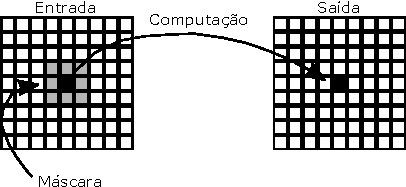
\includegraphics[width=0.6\textwidth]{26}
% 	\end{figure}
% \end{frame}

\begin{frame}\frametitle{\textit{Framework} PSkel}
    \subsection{Framework PSkel}

    \textbf{Objetivo}
    \begin{itemize}
        \item{Oferecer suporte para execução paralela de aplicações do padrão estêncil em ambientes heterogêneos (CPU e GPU)~\cite{pereira15}}
    \end{itemize}

    \vspace{0.5cm}

    \textbf{Funcionamento}
    \begin{itemize}
        \item {O usuário descreve o \textit{kernel} principal da computação estêncil}
        \item {O framework se encarrega de distribuir a computação na CPU e GPU}
        \item {Transferências de dados e particionamento de tarefas de maneira transparente}
    \end{itemize}
\end{frame}

\begin{frame}[fragile]
    \frametitle{\textit{Framework} PSkel}
    \begin{lstlisting}[style=highlight, gobble=4]
        __parallel__ void
        stencilKernel(Array2D<float> A, Array2D<float> B,
        Mask2D<int> mask, struct Arguments args,
        int x, int y){
            B(x,y) = args.alpha * (A(x,y+1) + A(x,y-1) +
            A(x+1,y) + A(x-1,y));
        }

        void main(){
            /* ... */
            Array2D<float> input(A,M,N);
            Array2D<float> output(B,M,N);
            int neighbors = {{0,1}, {-1,0}, {1,0}, {-1,0}};
            Mask2D<int> mask(4, neighbors);
            struct Arguments args(alpha, beta);
            /* ... */
            Stencil2D<Array2D<float>, Mask2D<int>, Arguments>
            jacobi(A,B,args);
            jacobi.runIterative(device::GPU, timesteps, 1.0);
            /* ... */
        }
    \end{lstlisting}
\end{frame}

\begin{frame}[fragile]
    \frametitle{\textit{Framework} PSkel}
    \begin{lstlisting}[style=base, gobble=4]
        @__parallel__ void
        stencilKernel(Array2D<float> A, Array2D<float> B,
        Mask2D<int> mask, struct Arguments args,
        int x, int y){
            B(x,y) = args.alpha * (A(x,y+1) + A(x,y-1) +
            A(x+1,y) + A(x-1,y));
        }
        @
        void main(){
            /* ... */
            @Array2D<float> input(A,M,N);
            Array2D<float> output(B,M,N);@
            @int neighbors = {{0,1}, {-1,0}, {1,0}, {-1,0}};
            Mask2D<int> mask(4, neighbors);@
            @struct Arguments args(alpha, beta);@
            /* ... */
            @Stencil2D<Array2D<float>, Mask2D<int>, Arguments>
            jacobi(A,B,args);
            jacobi.runIterative(device::GPU, timesteps, 1.0);@
            /* ... */
        }
    \end{lstlisting}
\end{frame}


\begin{frame}[fragile]
    \frametitle{\textit{Framework} PSkel}
    \begin{lstlisting}[style=highlight, gobble=4]
        __parallel__ void
        stencilKernel(Array2D<float> A, Array2D<float> B,
        Mask2D<int> mask, struct Arguments args,
        int x, int y){
            B(x,y) = args.alpha * (A(x,y+1) + A(x,y-1) +
            A(x+1,y) + A(x-1,y));
        }

        void main(){
            /* ... */
            Array2D<float> input(A,M,N);
            Array2D<float> output(B,M,N);
            int neighbors = {{0,1}, {-1,0}, {1,0}, {-1,0}};
            Mask2D<int> mask(4, neighbors);
            struct Arguments args(alpha, beta);
            /* ... */
            Stencil2D<Array2D<float>, Mask2D<int>, Arguments>
            jacobi(A,B,args);
            jacobi.runIterative(device::GPU, timesteps, 1.0);
            /* ... */
        }
    \end{lstlisting}
\end{frame}

\subsection{MPPA-256}
\begin{frame}\frametitle{MPPA-256}
    \textbf{Características}

    \begin{itemize}
        \item {Manycore de baixo consumo de energia}
        \item {256 núcleos organizados em 16 clusters}
        \item {4 subsistemas de E/S}
        \item {Comunicação feita por NoC \textit{torus} 2D}
    \end{itemize}

    % \begin{figure}
    \begin{center}
        \only<1>{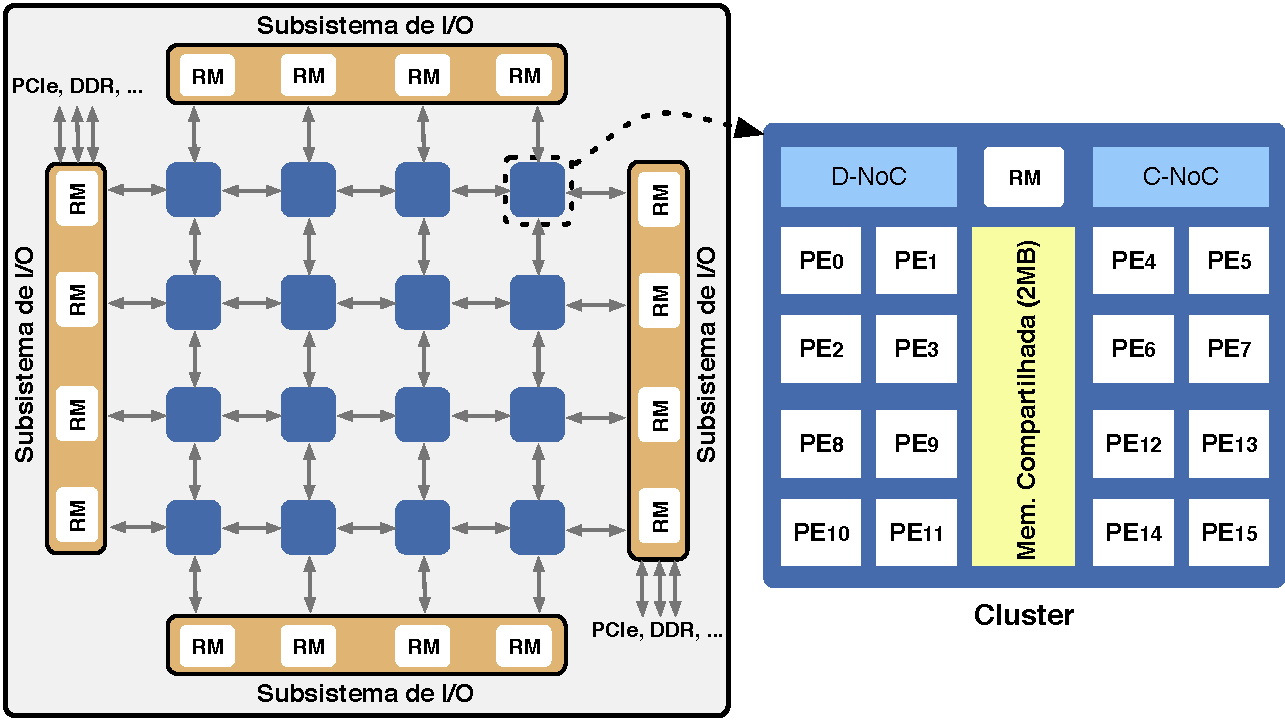
\includegraphics[width=0.80\textwidth]{25.pdf}}
        \only<2>{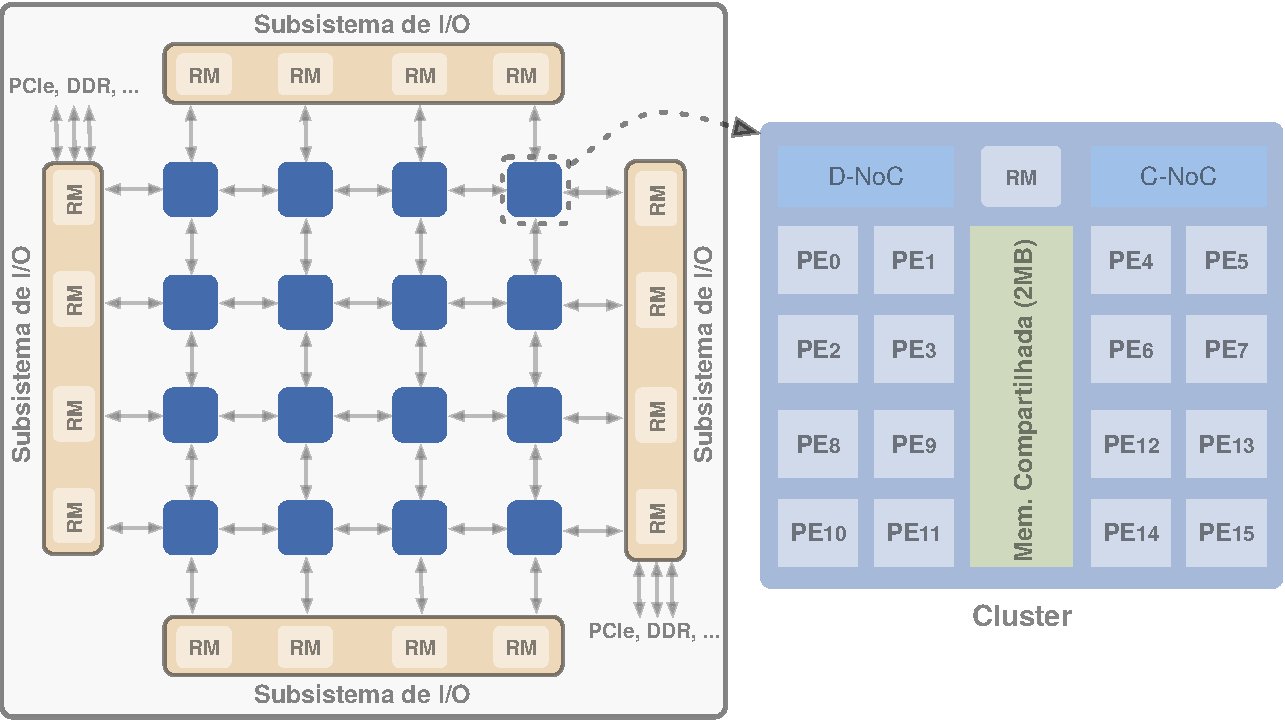
\includegraphics[width=0.80\textwidth]{cluster-overallMPPA.pdf}}%
        \only<3>{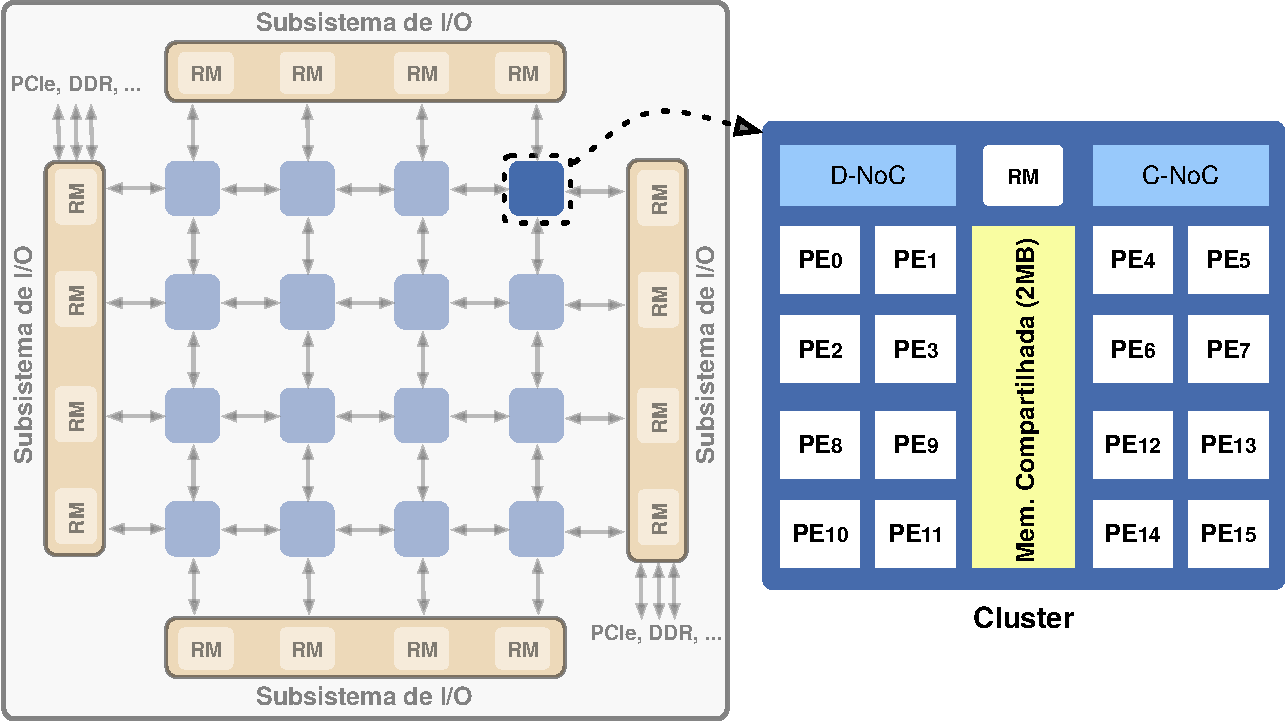
\includegraphics[width=0.80\textwidth]{clusterMPPA.pdf}}%
        \only<4>{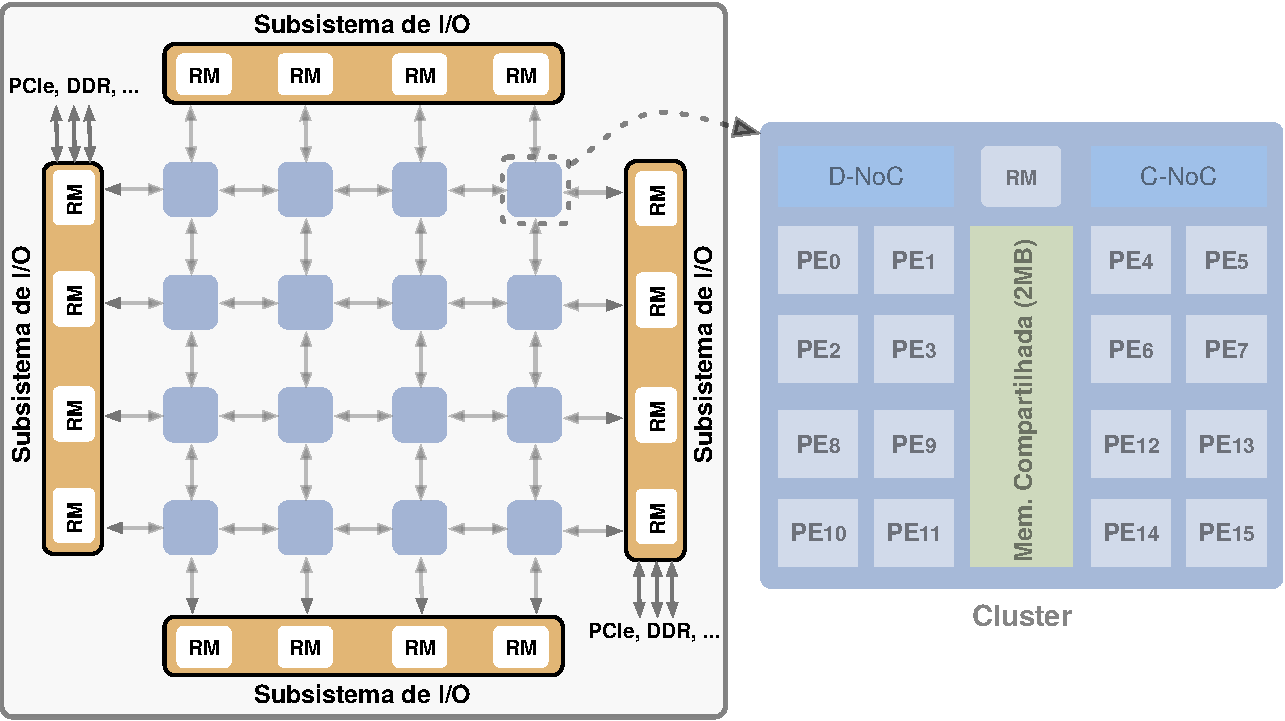
\includegraphics[width=0.80\textwidth]{io-overallMPPA.pdf}}
        \only<5>{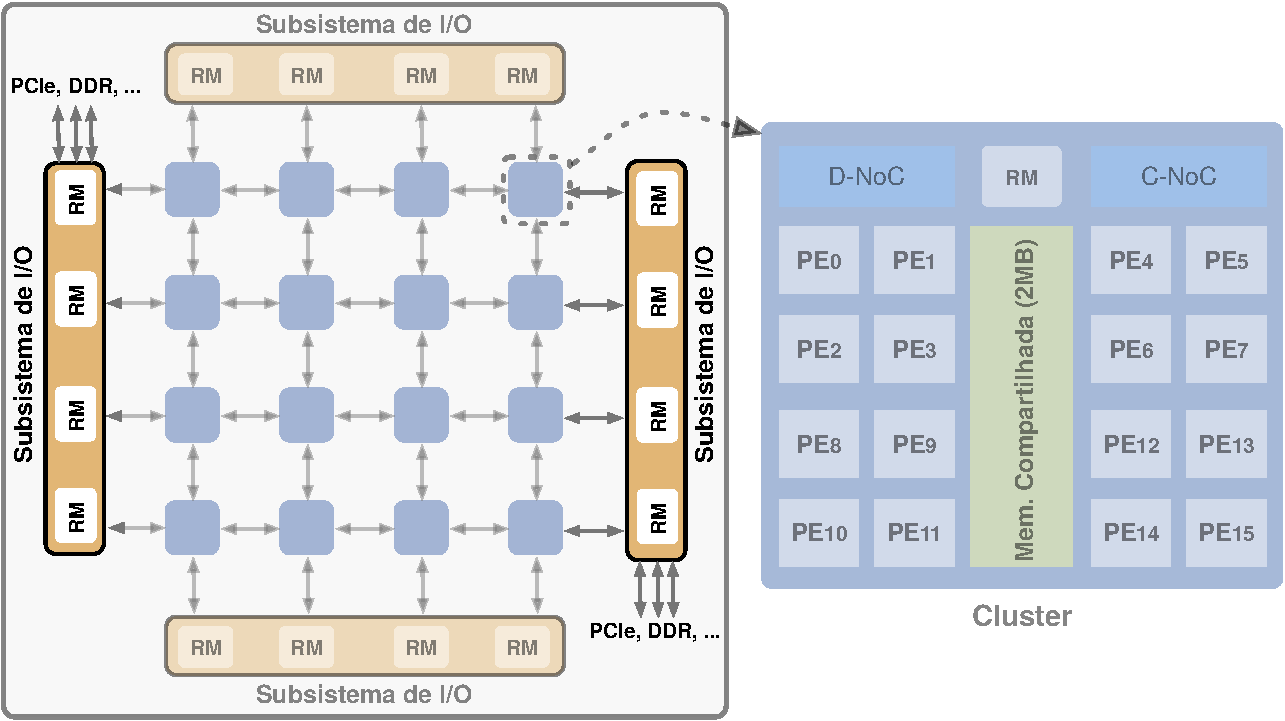
\includegraphics[width=0.80\textwidth]{ioConn-overallMPPA.pdf}}
        \only<6>{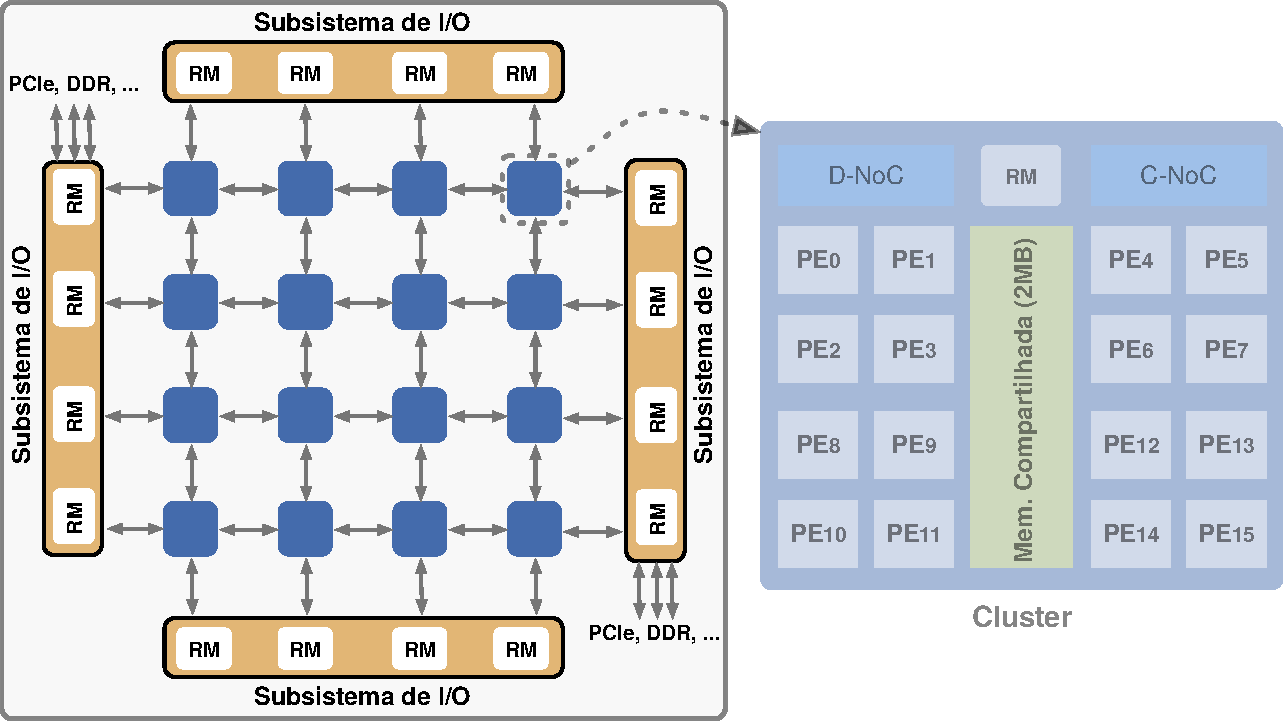
\includegraphics[width=0.80\textwidth]{conn-overallMPPA.pdf}}
        \only<7>{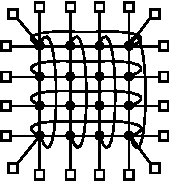
\includegraphics[width=0.42\textwidth]{topologia.pdf}}
    \end{center}
    % 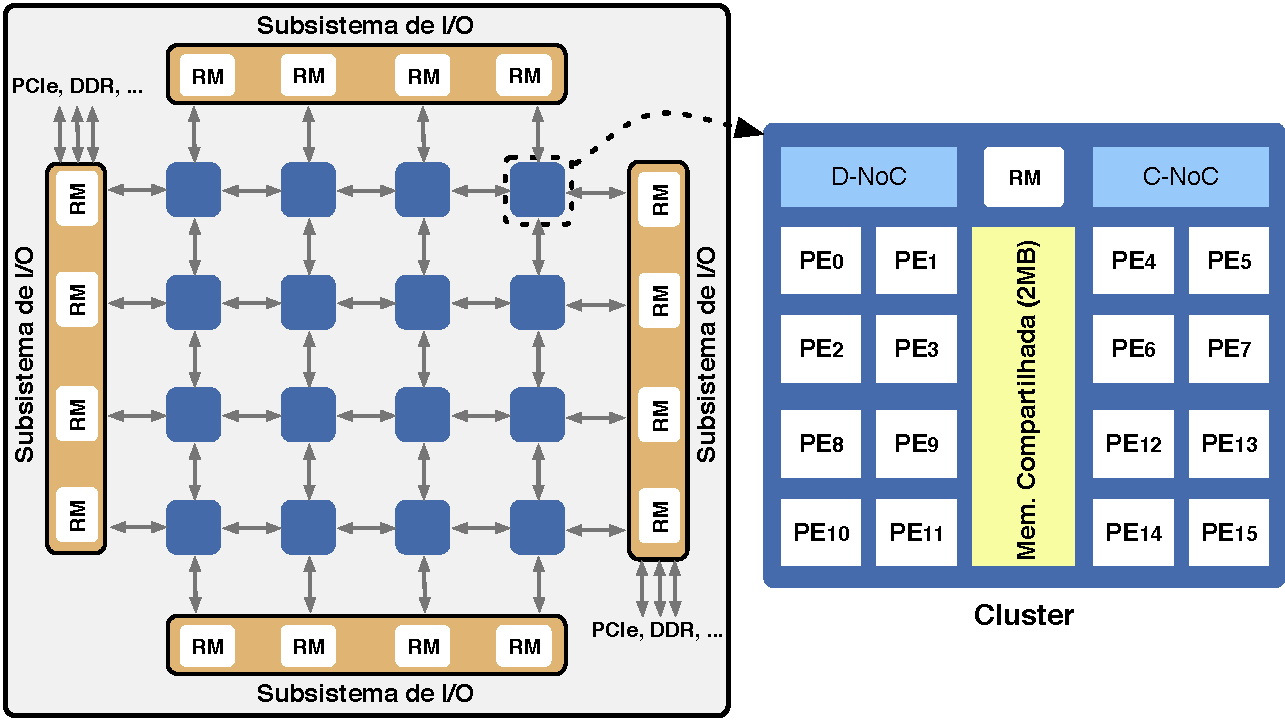
\includegraphics[width=0.65\textwidth]{25}
    % \end{figure}

\end{frame}

\begin{frame}\frametitle{MPPA-256}
    \textbf{Dificuldades encontradas no desenvolvimento de aplicações para o MPPA-256}

    \begin{itemize}
        \item \textbf{Comunicação via NoC}: toda a comunicação é feita através de uma API proprietária de baixo nível similar a \textit{POSIX Interprocess Communication (IPC)}
        \item \textbf{Memória limitada nos \textit{clusters}}: cada \textit{cluster} possui somente uma memória local de 2MB
        \item \textbf{Baixo nível de abstração}: toda a comunicação é gerenciada pelo desenvolvedor de maneira explícita
    \end{itemize}
\end{frame}


\section{Proposta}
\begin{frame}\frametitle{Proposta}
    \textbf{Objetivo Geral}
    \begin{itemize}
        \item {Adaptar o \Fw PSkel para o processador MPPA-256}
            % \begin{itemize}
                \item {Simplicar o desenvolvimento para o MPPA-256}
                \item {Desenvolvedor poderá aproveitar os benefícios do processador}
                \item {Aplicações desenvolvidas poderão ser portadas sem alteração}
            % \end{itemize}
    \end{itemize}
\end{frame}


\begin{frame}\frametitle{Proposta}
    \textbf{Objetivos Específicos}
    \begin{itemize}
        \item {Definir uma estratégia de distribuição de dados entre os \textit{clusters} do MPPA-256}
        \item {Propor e implementar técnicas que permitam reduzir os custos de comunicação na NoC}
        \item {Adaptar as principais classes e abstrações existentes no PSkel para o processador MPPA-256}
        \item {Realizar uma análise de desempenho e energia sobre a solução proposta}
        \item {Realizar comparações de desempenho e consumo de energia com um processador \textit{multicore} atual}
    \end{itemize}
\end{frame}


\section{Contribuições}
\begin{frame}\frametitle{Contribuições}
    % \begin{thebibliography}{1}
    % \setbeamertemplate{bibliography item}[text]
    % {\tiny \bibitem{E}
    %     PODESTA JUNIOR, E. ; PEREIRA, A. D. ; ROCHA, R. C. O. ; CASTRO,
    %         MÁRCIO ; GOES, L. F. W. \textbf{Execução Energeticamente Eficiente
    %             de Aplicações Estêncil com o Processador Manycore MPPA-256}. In:
    %         Simpósio em Sistemas Computacionais de Alto Desempenho (WSCAD),
    %         2017, Campinas, São Paulo.
    %     }
    % \end{thebibliography}
    \begin{itemize}
    {\tiny
        \item PODESTA JUNIOR, E. ; MARQUES, B. ; CASTRO, M. \textbf{Energy
                Efficient Stencil Computations on the Low-Power Manycore
                MPPA-256 Processor}. In: Conferência Européia Internacional de
            Computação Paralela e Distribuída (EURO-PAR), 2018, Turin, Itália.
        \item PODESTA JUNIOR, E. ; PEREIRA, A. D. ; ROCHA, R. C. O. ; CASTRO,
            MÁRCIO ; GOES, L. F. W. \textbf{Execução Energeticamente Eficiente
                de Aplicações Estêncil com o Processador Manycore MPPA-256}. In:
            Simpósio em Sistemas Computacionais de Alto Desempenho (WSCAD),
            2017, Campinas, São Paulo.

        \item PODESTA JUNIOR, E. ; PEREIRA, A. D. ; ROCHA, R. C. O. ; CASTRO, M.
            ; GOES, L. F. W. \textbf{Uma Implementação do Framework PSkel com
                Suporte a Aplicações Estêncil Iterativas para o Processador
                MPPA-256}. In: Escola Regional de Alto Desempenho do Estado do
            Rio Grande do Sul (ERAD/RS), 2017, Ijuí, Rio Grande do Sul.

        \item PODESTA JUNIOR, E. ; PEREIRA, A. D. ; PENNA, P. H. ; ROCHA, R. C.
            O. ; CASTRO, M. ; GOES, L. F. W. \textbf{PSkel-MPPA: Uma Adaptação
                do Framework PSkel para o Processador Manycore MPPA-256}. In:
            Escola Regional de Alto Desempenho do Estado do Rio Grande do Sul
            (ERAD/RS), 2016, São Leopoldo, Rio Grande do Sul.

    }
    \end{itemize}
\end{frame}

% \item {Implementação completa do \textit{framework} PSkel para o processador \textit{manycore} MPPA-256}
% \item {Suporte a aplicações estêncil iterativas}
% \item {Particionamento flexível dos dados entre os \textit{clusters} (\textit{tiles} de dimensão arbitrária)}

\section{Implementação}
\begin{frame}\frametitle{Implementação}
    \begin{itemize}
        \item {Modelo mestre/trabalhador}
        \item \textbf{Mestre (subsistema de I/O)}
            \begin{itemize}
                \item {Subdivide a matriz de entrada em \textit{tiles} e os envia sob demanda aos trabalhadores (\textit{clusters})}
                \item {Envio feito de acordo com o modelo \textit{Round-Robin}}
                \item {Particionamento flexível dos dados entre os \textit{clusters} (\textit{tiles} de dimensão arbitrária)}
                % \item {Computações redundantes devido à técnica de \textit{tiling} trapezoidal}
                % \item {Redução no número de comunicações}
            \end{itemize}
    \end{itemize}
\end{frame}


\begin{frame}\frametitle{Implementação}
    \textbf{Trabalhador (\textit{cluster})}
    \begin{itemize}
        \item {Recebe o \textit{tile}, realiza a computação do \textit{kernel} estêncil sobre o \textit{tile} e envia a reposta ao mestre}
            \item {Computação realizada por meio de diretivas OpenMP}
        \item {Repete a computação para cada \textit{tile} atribuído pelo mestre}
        % \item {Possibilidade de realizar várias iterações sobre o mesmo \textit{tile}}
        % \item {Melhoria do desempenho}
    \end{itemize}
\end{frame}

\begin{frame}\frametitle{Problema}
    \begin{itemize}
        \item {No padrão estêncil temos computações iterativas}
        \item {Grande número de comunicações entre o processo mestre e trabalhador}
        \item {Atribuir parte das iterações para o processo trabalhador}
        \item {Redução no número de comunicações}
    \end{itemize}
\end{frame}

\begin{frame}\frametitle{\textit{Tiling} Trapezoidal}
    \begin{flushleft}
        \only<1>{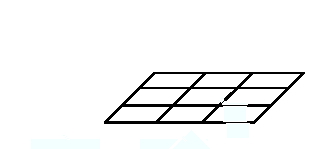
\includegraphics[width=0.80\textwidth]{tiling1.pdf}}
        \only<2>{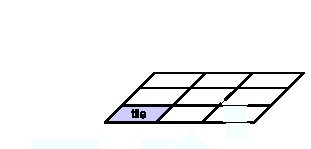
\includegraphics[width=0.80\textwidth]{tiling2.pdf}}
        \only<3>{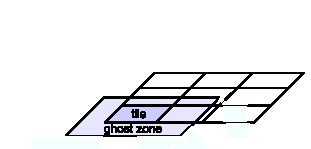
\includegraphics[width=0.80\textwidth]{tiling3.pdf}}
        \only<4>{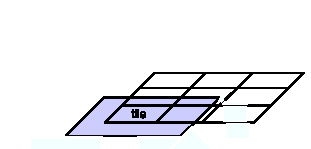
\includegraphics[width=0.80\textwidth]{tiling4.pdf}}
        \only<5>{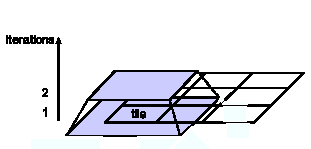
\includegraphics[width=0.80\textwidth]{tiling5.pdf}}
        \only<6>{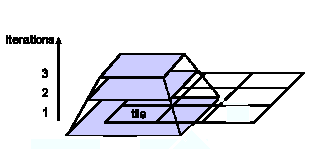
\includegraphics[width=0.80\textwidth]{tiling6.pdf}}
        \only<7>{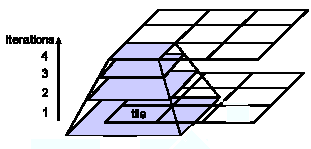
\includegraphics[width=0.80\textwidth]{tiling7.pdf}}
        \only<8>{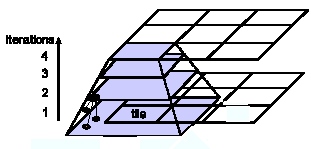
\includegraphics[width=0.80\textwidth]{tiling8.pdf}}
    \end{flushleft}
\end{frame}

\begin{frame}\frametitle{Comunicação}
    \begin{flushleft}
        \only<1>{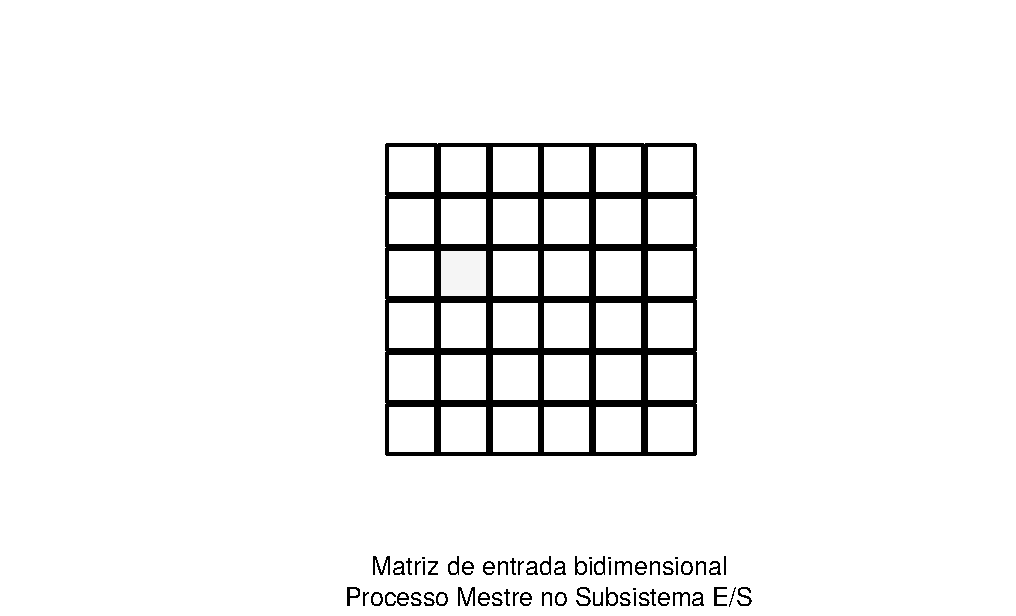
\includegraphics[width=10cm]{stridesImageSlide1.pdf}}
        \only<2>{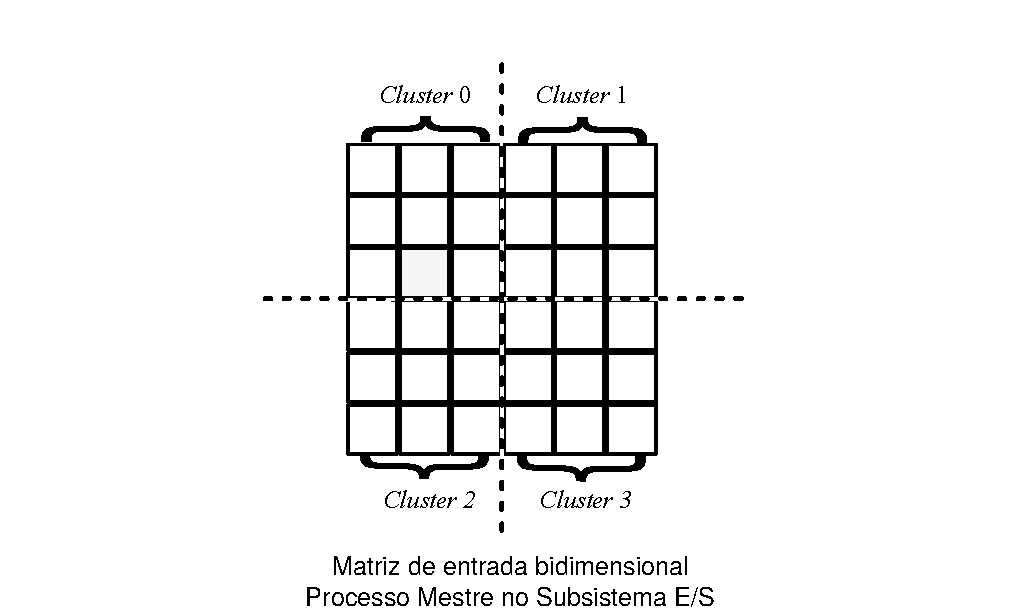
\includegraphics[width=10.3cm]{stridesImageSlide2.pdf}}
        \only<3>{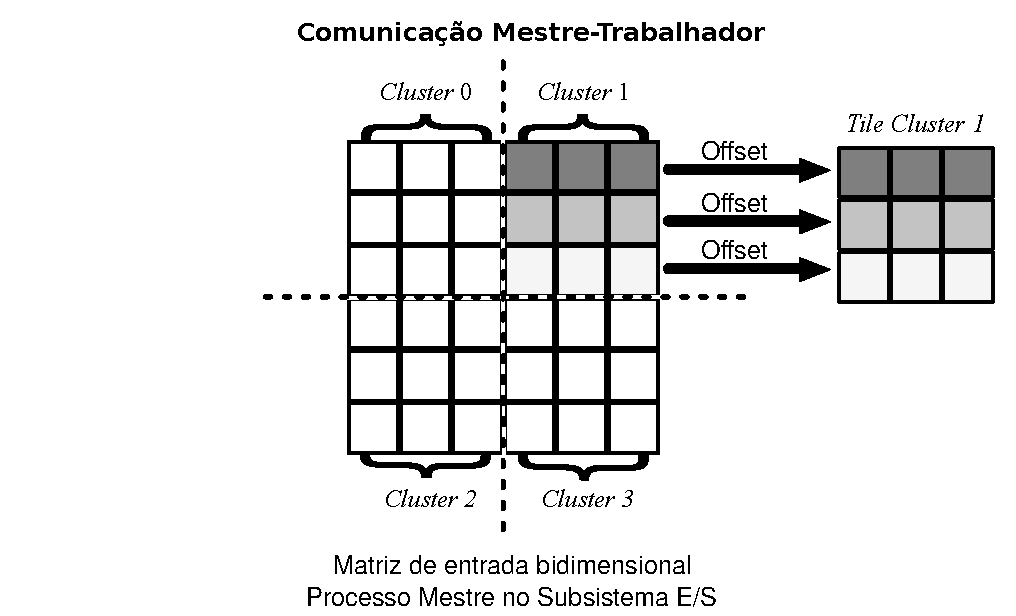
\includegraphics[width=10.3cm]{stridesImageSlide3.pdf}}
        \only<4>{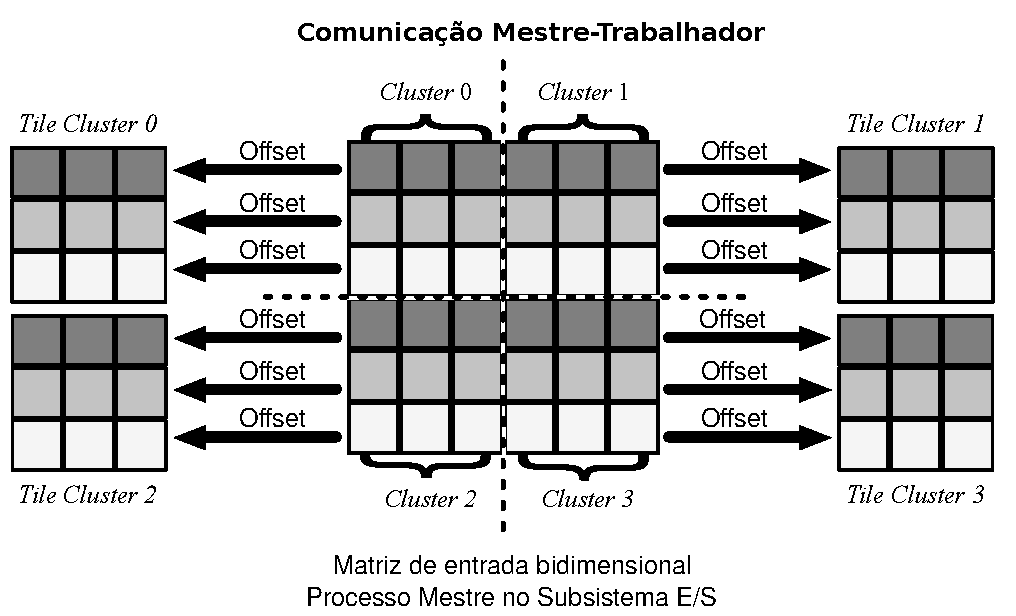
\includegraphics[width=10.3cm]{stridesImageSlide4.pdf}}
        \only<5>{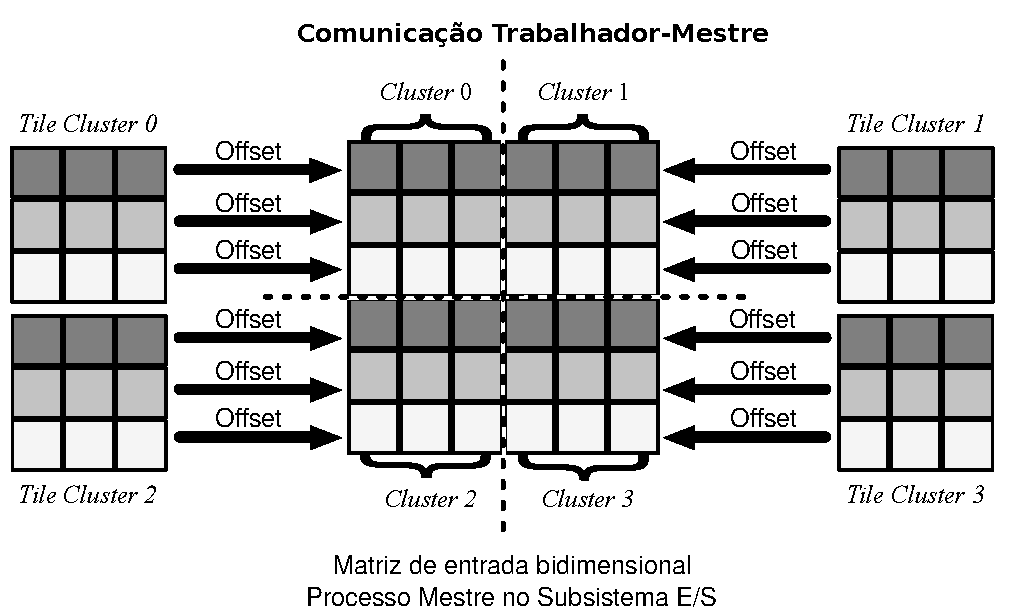
\includegraphics[width=10.3cm]{stridesImageSlide5.pdf}}
    \end{flushleft}
\end{frame}


\section{Resultados}
\begin{frame}\frametitle{Resultados}
    \begin{itemize}
        \item{\textbf{Processador \textit{manycore} MPPA-256}}
            \begin{itemize}
                \item{Calculado a média do tempo e energia gastos sobre 5 execuções}
                \item{Baixa variabilidade entre execuções}
            \end{itemize}
        \item{\textbf{Processador \textit{multicore} Intel Xeon E5-2640 v4}}
            \begin{itemize}
                \item{Calculado a média do tempo e energia gastos sobre 30 execuções}
            \end{itemize}
        \item{Desvio padrão menor que 1$\%$}
        \item{Todos os experimentos utilizaram 30 iterações}
    \end{itemize}
\end{frame}

\begin{frame}\frametitle{Resultados}
    \begin{itemize}
        \item \textbf{Aplicações}
            \begin{itemize}
                \item \textbf{Fur:} simulação de padrões de pigmento em pelos de animais~\cite{Castro-Podesta-ERAD:2016}
                \item\textbf{GoL:} autômato celular que implementa o Jogo da Vida de Conway~\cite{pereira15}
                \item\textbf{Jacobi:} método iterativo de Jacobi para a resolução de equações matriciais~\cite{pereira15}
            \end{itemize}
    \end{itemize}
\end{frame}

\begin{frame}\frametitle{Resultados}
    \textbf{Teste de Escalabilidade}
    \begin{itemize}
        \item Matriz: 2048x2048
        \item \textit{Tile:} 128x128
    \end{itemize}
    \begin{figure}
        \centering
        \begin{subfigure}{\textwidth}
            \centering
            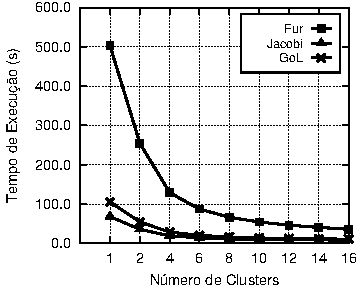
\includegraphics[width=0.50\textwidth]{figs/MPPAPlotScalability.pdf}
            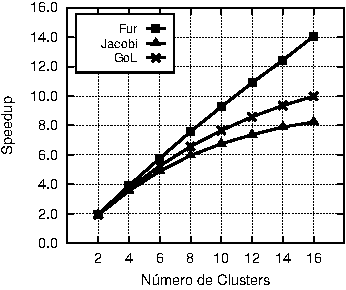
\includegraphics[width=0.49\textwidth]{figs/MPPAPlotSpeedup.pdf}
        \end{subfigure}
    \end{figure}
\end{frame}

\begin{frame}\frametitle{Resultados}
    \textbf{Tamanho dos \textit{tiles} vs. Desempenho}
    %	\begin{figure}
    %		\centering
    %		\subfigure 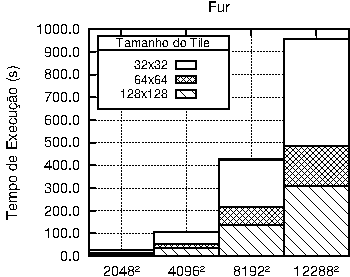
\includegraphics[width=0.27\textwidth]{figs/MPPAPlotfurTimeTiles.pdf}
    %		\qquad
    %		\subfigure 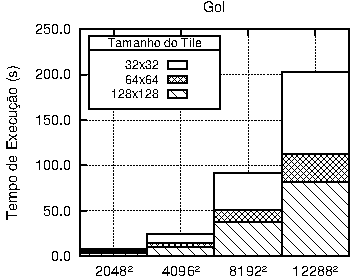
\includegraphics[width=0.27\textwidth]{figs/MPPAPlotgolTimeTiles.pdf}
    %   	\qquad
    %	\subfigure 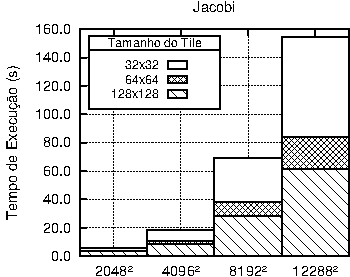
\includegraphics[width=0.27\textwidth]{figs/MPPAPlotjacobiTimeTiles.pdf}
    %	\end{figure}

    %	\begin{figure}
    %	    \centering
    %		\subfigure 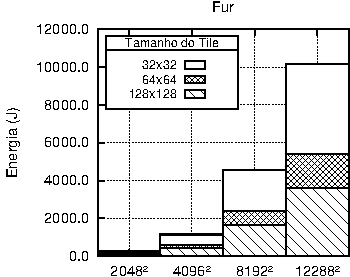
\includegraphics[width=0.27\textwidth]{figs/MPPAPlotfurEnergyTiles.pdf}
    %		\qquad
    %		\subfigure 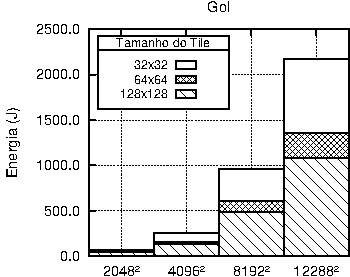
\includegraphics[width=0.27\textwidth]{figs/MPPAPlotgolEnergyTiles.pdf}
    %   	\qquad
    %	\subfigure 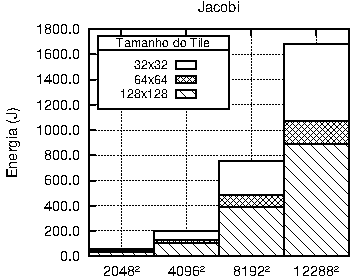
\includegraphics[width=0.27\textwidth]{figs/MPPAPlotjacobiEnergyTiles.pdf}
    %\end{figure}
    \begin{itemize}
    \item 16 \textit{clusters} utilizados
    \end{itemize}
    \begin{figure}
        \centering
        \only<1>{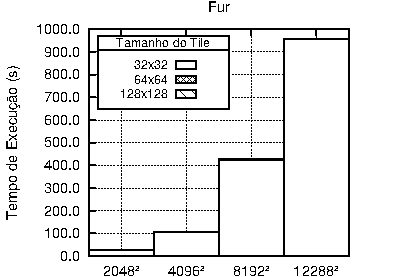
\includegraphics[width=.70\textwidth]{figs/MPPAPlotfurTimeTiles1.pdf}}
        \only<2>{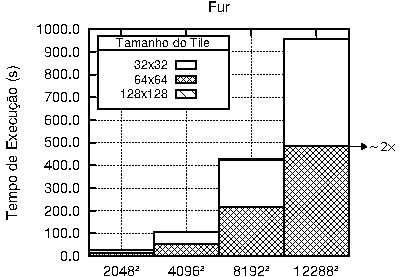
\includegraphics[width=.70\textwidth]{figs/MPPAPlotfurTimeTiles2.pdf}}
        \only<3>{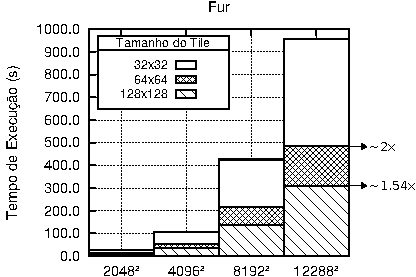
\includegraphics[width=.70\textwidth]{figs/MPPAPlotfurTimeTiles3.pdf}}
    \end{figure}
\end{frame}


\begin{frame}\frametitle{Resultados}
    \textbf{Tamanho dos \textit{tiles} vs. Energia}
    \begin{itemize}
    \item 16 \textit{clusters} utilizados
    \end{itemize}
    \begin{figure}
        \centering
        \only<1>{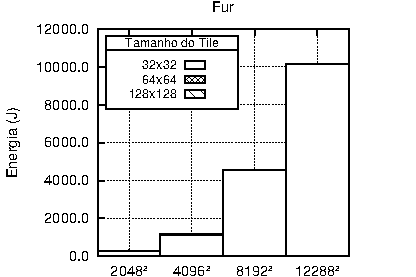
\includegraphics[width=.70\textwidth]{figs/MPPAPlotfurEnergyTiles1.pdf}}
        \only<2>{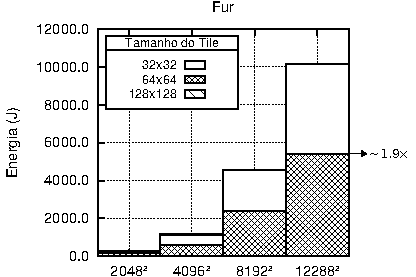
\includegraphics[width=.70\textwidth]{figs/MPPAPlotfurEnergyTiles2.pdf}}
        \only<3>{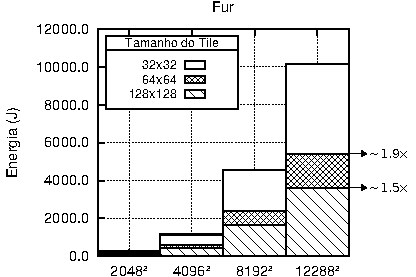
\includegraphics[width=.70\textwidth]{figs/MPPAPlotfurEnergyTiles3.pdf}}
    \end{figure}
\end{frame}

\begin{frame}\frametitle{Resultados}
    \textbf{MPPA vs. Intel Xeon}
	\begin{itemize}
	\item Matriz: 12288x12288
    \item \textit{Tile}: 128x128
    \item 16 \textit{clusters} utilizados no MPPA
    \item 10 \textit{threads} sem \textit{hyperthreading} utilizadas no Intel Xeon
	\end{itemize}
\end{frame}

\begin{frame}\frametitle{Resultados}
    % 	\begin{figure}
    % 		\centering
    % 		\begin{subfigure}{.45\textwidth}
    % 	  		\centering
    % 	  		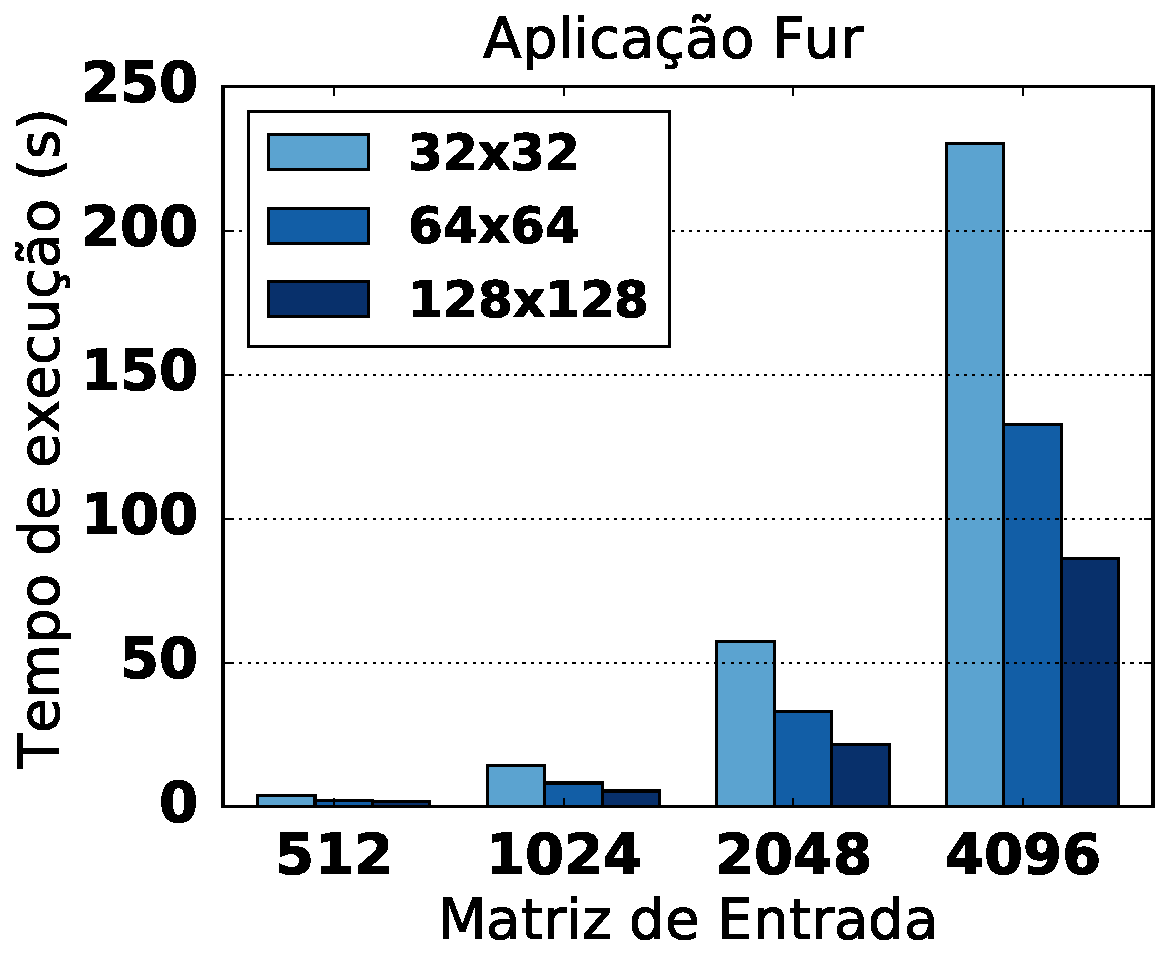
\includegraphics[width=.7\textwidth]{10}
    % 		\end{subfigure}%
    % 		\begin{subfigure}{.45\textwidth}
    % 	  		\centering
    % 	  		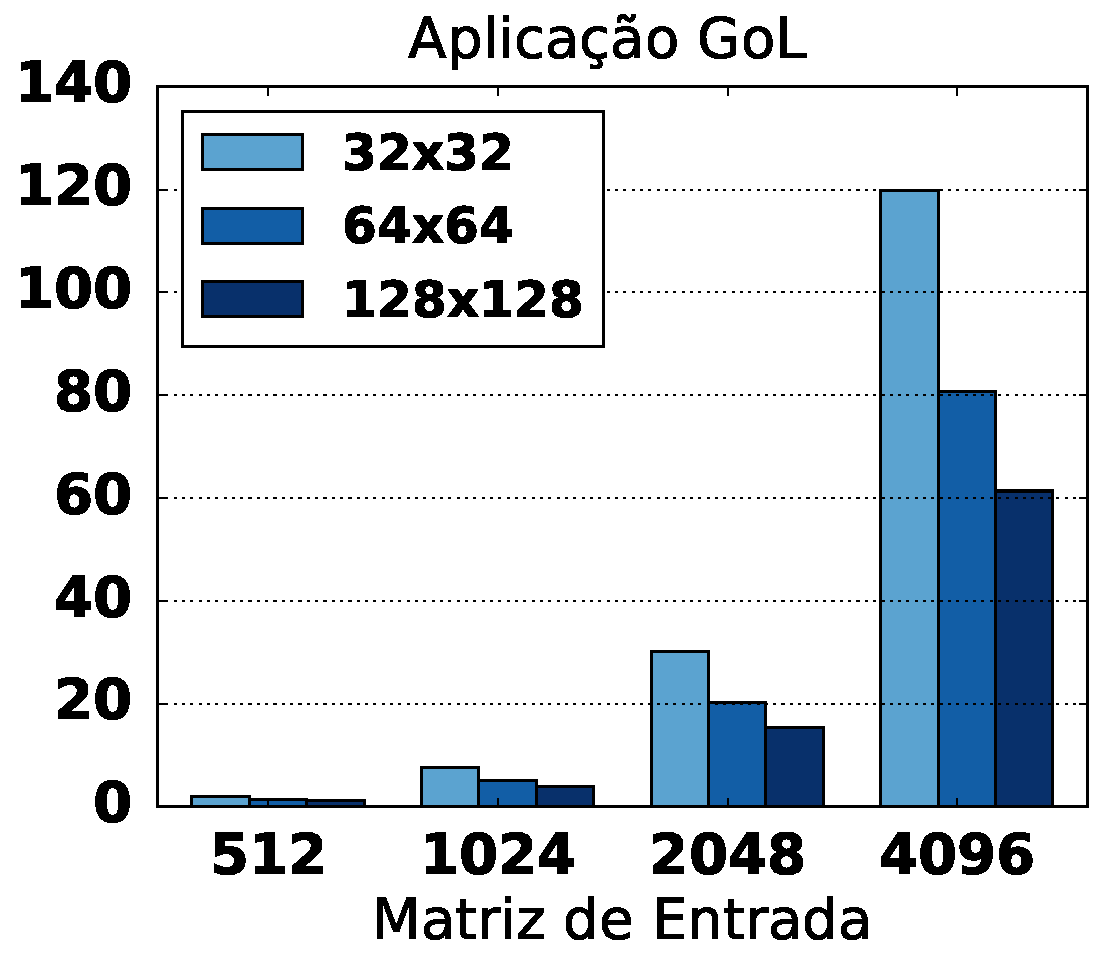
\includegraphics[width=.7\textwidth]{14}
    % 		\end{subfigure}%
    %         \begin{subfigure}{.45\textwidth}
    % 	  		\centering
    % 	  		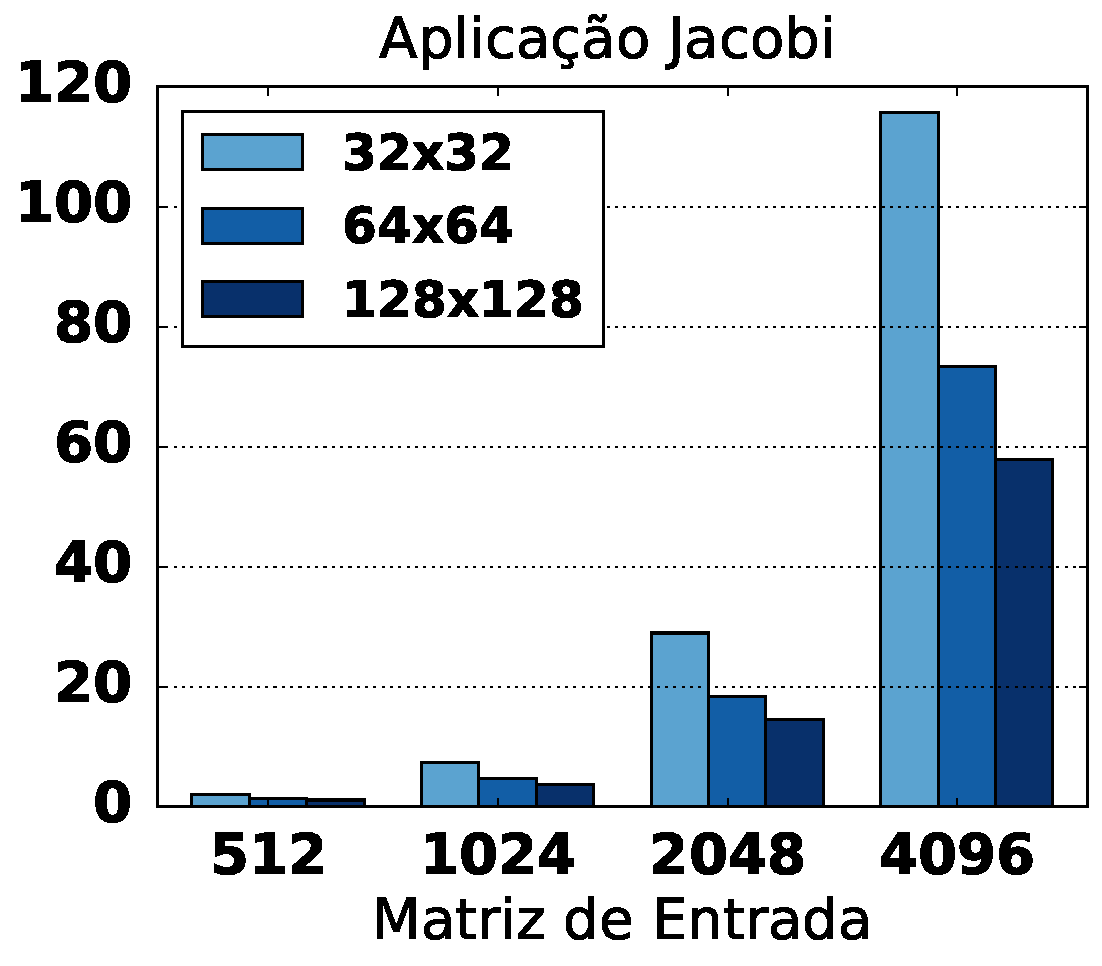
\includegraphics[width=.7\textwidth]{18}
    % 		\end{subfigure}
    % 	\end{figure}
    \textbf{MPPA vs. Intel Xeon}
    \begin{figure}

        \centering
        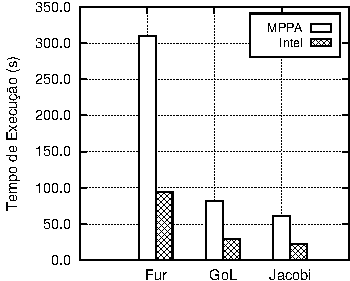
\includegraphics[width=.49\textwidth]{figs/ComparisonTimeTiles10.pdf}
        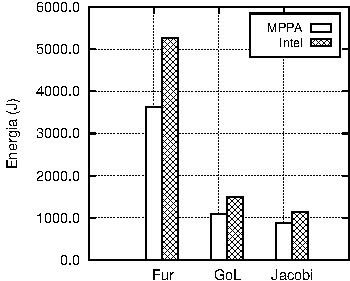
\includegraphics[width=.49\textwidth]{figs/9.pdf}

    \end{figure}
    \begin{itemize}
    \item Para as aplicações Fur, GoL e Jacobi:
    \begin{itemize}
    \item O Intel Xeon é 3.30x, 2.83x e 2.69x, respectivamente, mais rápido
    \item O MPPA consome 1.45x, 1.38x e 1.27x, respectivamente, menos energia
    \end{itemize}
    \end{itemize}


\end{frame}

%\begin{frame}\frametitle{Resultados}
%    \begin{figure}

%    \end{figure}
%\end{frame}

\section{Conclusões e Trabalhos Futuros}
\begin{frame}\frametitle{Conclusões}
    \begin{itemize}
        \item A adaptação apresenta uma eficiência energética superior ao Intel Xeon
        \item A adaptação demonstrou um bom potencial
        \item A comunicação tem impacto sobre o tempo e energia obtidos
        \item Boa escalabilidade em relação à variação dos \textit{clusters} e variação do tamanho dos \textit{tiles}
    \end{itemize}

    \vspace{0.5cm}

    \textbf{Trabalhos Futuros}
    \begin{itemize}
        \item Realizar experimentos com estruturas tridimensionais
        \item Reduzir os sobrecustos de comunicação
        \item Comparar a adaptação com outros processadores embarcados
    \end{itemize}
\end{frame}

%Fim
\begingroup
    \makeatletter
    \setlength{\hoffset}{-.5\beamer@sidebarwidth}
    \makeatother
    \begin{frame}[plain,t,noframenumbering]
        \titlepage
    \end{frame}
\endgroup

\section{Referências}
\begin{frame}\frametitle{Referências}
    {\tiny
        \bibliographystyle{apalike}
        \bibliography{bibliografia}}
\end{frame}

% \section{Extra}
% \begin{frame}\frametitle{Extra}
% \begin{figure}[t]
%   \begin{minipage}[b]{0.9\textwidth}
% 	\centering
%     % \caption{\textit{tiling} 2D.}
%     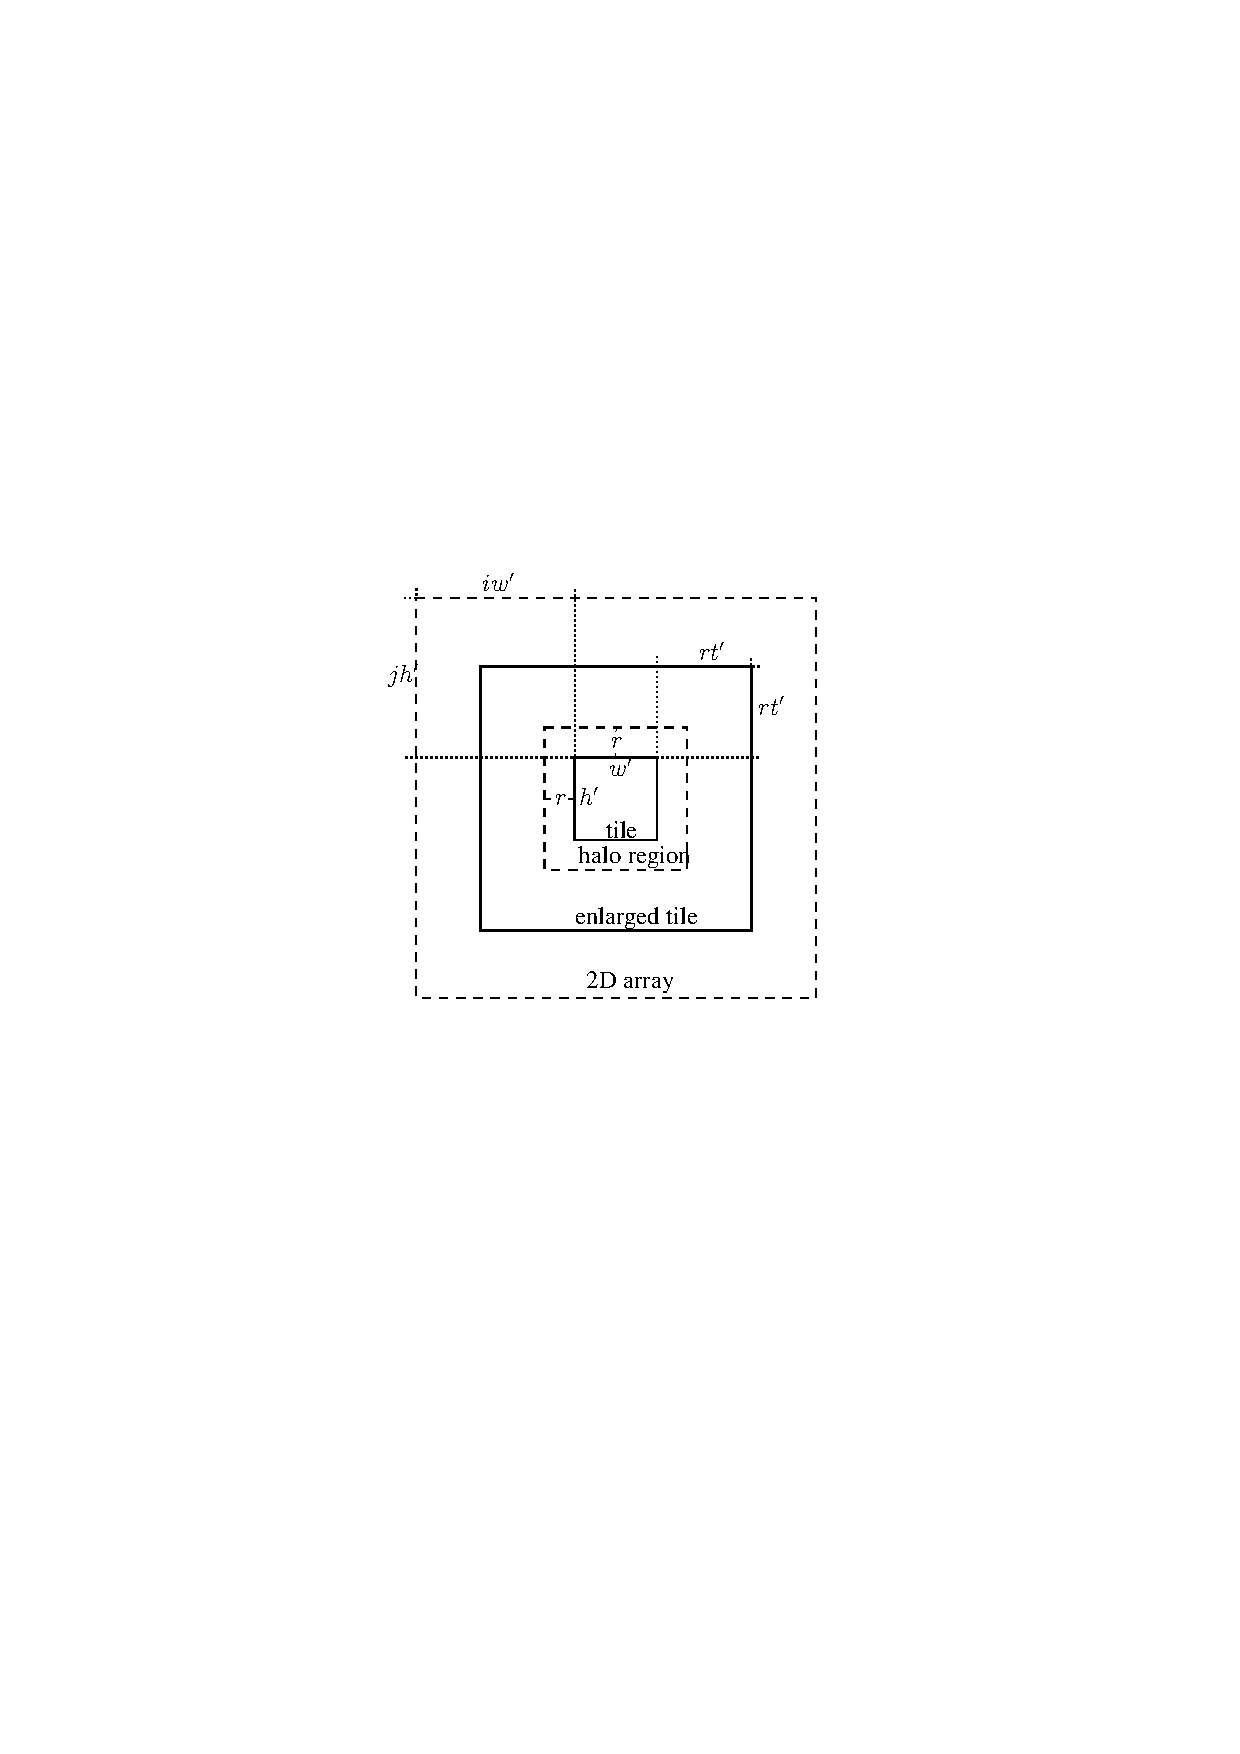
\includegraphics[height=5cm]{figs/tile.pdf} \\
%     % Fonte:~\cite{rocha17}
% 	\label{fig:block2d}
%   \end{minipage}
% \end{figure}
% \end{frame}

\end{document}
